%=========================================================================
% Start of activity on simple harmonic motion.
%=========================================================================
\preClass{Derivatives of Basic Trigonometric Functions}

\begin{problem}
\item Determine the derivatives of the following functions:
  \begin{subproblem}
  \item $\sin(3t)$
    \vfill
  \item $\cos(8t)$
    \vfill
  \end{subproblem}
\item Determine the general anti-derivatives of the following functions:
  \begin{subproblem}
  \item $\cos(3t)$
    \vfill
  \item $\sin(8t)$
    \vfill
  \end{subproblem}

\clearpage

\item An object has an acceleration given by
  \begin{eqnarray*}
    a(t) & = & 2\sin(5t) + 5e^{-2t},
  \end{eqnarray*}
  and the initial velocity is $v_0$, and the initial position is $x_0$.
  \begin{subproblem}
  \item Determine the position at any time.
    \vfill
  \item Describe the qualitative behaviour of the object's
    position. Does the object's position oscillate, grow, or decay?
    For what values of $v_0$ and $x_0$ do you see different
    behaviours?
    \vfill
  \end{subproblem}

\end{problem}


\actTitle{Simple Harmonic Motion}
\begin{problem}

\item An object is attached to a rigid spring on a frictionless
  horizontal table. The origin is defined to be the equilibrium
  position for the object. The mass of the object is 3kg. The object
  is drawn back 0.05m and released from rest. The spring obeys Hooke's
  law, and it's constant is $k=0.4$N/m.
  \begin{subproblem}
    \item Make a sketch of the physical situation.
      \vfill
    \item Make a sketch of the free body diagram. Ignore any friction
      assuming that the friction is negligible for now.
      \vfill
    \item Describe the qualitative behaviour that you expect to see
      from the physical system. How should it behave? 
      \vfill
    \item Determine the equation of motion in the $x$-direction
      ignoring friction.
      \label{subproblem:odeMassSpring}
      \vfill

    \item Based on your description of the expected behaviour what
      kind of \textbf{functions} mimics that behaviour?
      \vspace{3em}

      \clearpage

    \item Assume that the solution has the form
      \begin{eqnarray*}
        x(t) & = & A \sin(\omega t) + B \cos(\omega t),
      \end{eqnarray*}
      where $A$, $B$, and $\omega$ are constants.
      \sideNote{It is not uncommon to just make a guess at a general
        form, and then check to see if your intuition is consistent
        with the equation.}
      \begin{subproblem}
      \item Determine the velocity and acceleration based on the
        definition of the position above.
        \vfill
      \item Substitute these results into your equation for the motion
        of the object you derived in question
        \ref{subproblem:odeMassSpring}.
        \vfill
        \clearpage
      \item Put all of the sines on one side of the equality and all
        of the cosines on the other side of the equality. What must be
        true about the left and right hand sides?
        \sideNote{Hint: It has to be true for \textbf{all} time!}
        \vspace{6em}
      \item Is it possible to determine values for the constants to
        satisfy the equation and the initial conditions? If so what
        are they?
        \sideNote{Hint: Yes.}
        \vfill
      \end{subproblem}

  \end{subproblem}
\end{problem}

\postClass

\begin{problem}
\item Briefly state two ideas from today's class.
  \begin{itemize}
  \item
  \item
  \end{itemize}
\item Determine the first and second derivatives of the following functions.
  \begin{subproblem}
  \item $8\sin(5t)$
    \vfill
  \item $23\cos(2t)$
    \vfill
  \item $8\sin(5t)+2\cos(5t)$
    \vfill
  \item $23\cos(2t)-14\sin(2t)$
    \vfill
  \end{subproblem}
  %\clearpage
  \item An object is attached to a rigid spring on a frictionless
    horizontal table. The origin is determined to be the equilibrium
    position for the object. The mass of the object is 4kg. The object
    is drawn back 0.1m and released from rest. The spring obeys Hooke's
    law with a constant, $k=0.5$N/m. Determine the position of the object
    at any time.
  \item An object is attached to a rigid spring on a frictionless
      horizontal table. The origin is determined to be the equilibrium
      position for the object. The mass of the object is 2kg. The object
      starts at the origin with an initial velocity of 3 m/sec.
      The spring obeys Hooke's law with a constant, $k=0.2$N/m.
      Determine the position of the object at any time.
\end{problem}

%=========================================================================
% Start of activity on finding optimal values of a parameter in SHM
%=========================================================================
\preClass{Simple Harmonic Motion}

\begin{problem}
\item Determine the solution to the following differential equations.
  \begin{subproblem}
  \item $x'' + 4 x  =  0$, $x(0)=0$, $v(0)=1$.
    \vfill
  \item $x'' + 8 x  =  0$, $x(0)=1$, $v(0)=0$.
    \vfill
  \end{subproblem}
\end{problem}


\actTitle{Optimization For Simple Harmonic Motion - Determining The System}
\begin{problem}
\item A spring mass system is to be constructed. The system will be
  assembled on a horizontal table, and friction is ignored.
  \begin{subproblem}
    \item Make a sketch of the physical situation.
      \vfill
    \item Make a sketch of the free body diagram.  Assume that the
      friction is negligible for now. Assume that the spring constant
      is $k$ N/m and the mass is $m$ 
      \vfill
    \item Describe the qualitative behaviour that you expect to see
      from the physical system. How should it behave?
      \vfill
    \item Determine the equation of motion ignoring friction.
      \vfill
  \end{subproblem}

  \clearpage

\item We now have the general equations of motion for a spring-mass
  system with parameters $k$ and $m$. The goal is to determine values
  of $k$ and $m$ so that the first time \textbf{after} $t=0$ the
  system will reach its maximum distance away from the origin in
  $t=0.1$ seconds. Assume that the object is first pulled 0.3 m from
  equilibrium and released from rest. What is the constraint for $k$
  and $m$?

  \vfill

\item The cost of the spring depends on $k$ and is $(1+k^2)$\$. The cost of
  the object depends on its mass and is ($m-2k)$\$. What is the
  total cost of building the system?

  \vspace{4em}

\item Formally express the cost and objective functions:
    \label{activity:optimization:spring}
    \begin{eqnarray*}
      \mathrm{Minimize:} & &  \\
      \mathrm{Constraint:} & &
    \end{eqnarray*}



\end{problem}


\postClass

\begin{problem}
\item Briefly state two ideas from today's class.
  \begin{itemize}
  \item
  \item
  \end{itemize}


\item Rewrite the system to optimize from this set of activities
  (question \ref{activity:optimization:spring}).
    \begin{eqnarray*}
      \mathrm{Minimize:} & &  \\
      \mathrm{Constraint:} & &
    \end{eqnarray*}
    \begin{subproblem}
    \item Make a sketch of the constraint.  \sideNote{ Be sure to
        label your axes and label all important points on your graph.}

      \vfill

    \item Add a sketch of the cost functions for various values of the
      cost. What is the general pattern? Make a prediction for the
      optimal values of $k$ and $m$.

      \vspace{3em}
    \end{subproblem}
\clearpage

\item Rewrite the system to optimze from this set of activities
  (question \ref{activity:optimization:spring}).
  \begin{eqnarray*}
    \mathrm{Minimize:} & &  \\
    \mathrm{Constraint:} & &
  \end{eqnarray*}

  \begin{subproblem}
  \item Analytically determine the optimal values of $k$ and $m$.
    \vfill
  \end{subproblem}
\end{problem}

%=========================================================================
% Start of activities on systems of equations
%=========================================================================
\preClass{Linearizations}

\begin{problem}
\item We examine the linearization of the function
  \begin{eqnarray*}
    f(x) & = & x^2-4.
  \end{eqnarray*}
  \begin{subproblem}
  \item Draw a set of axes where $-2\leq x \leq 2$.

    \sideNote{ Be sure to label your axes and label all important
      points on your graph.}

    \vfill

  \item Make a sketch of the function $f(x)$ on the axes.
  \item Add a sketch of the tangent line to the function at $x=1$.
  \item Determine the formula for the tangent line at $x=1$.
    \sideNote{Another term for the tangent line is the
      \textit{linearization}. The function you just found is the
      linearization of $f(x)$ at $x=1$.}
    \vfill

    (over)
  \end{subproblem}
  \clearpage
\item Determine the linearization of the function
  \begin{eqnarray*}
    g(t) & = & \cos(t)
  \end{eqnarray*}
  at $t=\frac{\pi}{4}$.
\end{problem}


\actTitle{Approximating Solutions to Nonlinear Equations}
\begin{problem}
\item We will examine a way to determine an estimate for the value of
  $x$ that satisfies $0=x^2-4$.
  \begin{subproblem}
  \item Draw a set of axes where $-2\leq x \leq 2$.

    \sideNote{ Be sure to label your axes and label all important
      points on your graph.}

    \vfill

  \item Make a sketch of the relationship $f(x)=x^2-4$ on the axes.
  \item Suppose you cannot determine the value of $x$ where $f(x)=0$,
    but you estimate that $x=1$ is close to a root. Add a sketch of
    the tangent line to the function at $x=1$.

  \item Mark the point where the height of the graph of the
    \textbf{tangent line} is zero. Is this new $x$ value a better or
    worse approximation for the value of the actual root?

    \vspace{2em}

    \clearpage


  \item Determine analytically the equation for the tangent line to
    the graph of the curve at the initial estimate for the root,
    $x=1$. Determine the value of $x$ where the height of the graph of
    the tangent line is zero.

    \vfill


  \item Add sketch of another tangent line at the new value of $x$ to
    your original plot on the previous page.

  \item Mark the point where the height of the \textbf{tangent line}
    is zero. Is this new $x$ value a better or worse approximation for
    the value of $x$?

    \vspace{2em}

  \item Determine analytically the tangent line to the graph of the
    curve at the new estimate for the root. Determine the value of $x$
    where the height of the graph of this new tangent line is zero.

    \vfill


  \item Add sketch of another tangent line at the new value of $x$ to
    your original plot on the previous page.

  \item Mark the point where the height of the graph of the
    \textbf{new tangent line} is zero. Is this new $x$ value a better
    or worse approximation for the value of $x$?


  \end{subproblem}

  \clearpage

\item Determine an algorithm to calculate the tangent line to a
  function at $x=a$, and find the value of $x$ where the height of the
  graph of the tangent line is zero.

  \vfill

\clearpage

\item Use your algorithm multiple times to find an approximation to
  the square root of 4 with an initial estimate of $x=1$.

  \vfill

\item How do you know when to stop applying the algorithm and your
  approximation is ``close?''

\end{problem}


\postClass

\begin{problem}
\item Briefly state two ideas from today's class.
  \begin{itemize}
  \item
  \item
  \end{itemize}
\item Graphically determine the values of $x$ and $y$ that satisfy
  both of the following equations:
  \begin{eqnarray*}
    x^2 + y  & = & 0, \\
    x - 2y^2 & = & 1.
  \end{eqnarray*}

  \begin{subproblem}
  \item Draw a set of axes where $-3\leq x \leq 3$ and $-3 \leq y \leq
    3$.

    \sideNote{ Be sure to label your axes and label all important
      points on your graph.}

    \vfill

  \item Make a sketch of the relationship $x^2+y=0$ on the axes.
  \item Make a sketch of the relationship $x-2y^2=1$ on the axes.
  \item Circle and estimate the points where both relationships are
    satisfied.
  \end{subproblem}
\clearpage
\item Determine the values of $x$ and $y$ that satisfy both of the
  following equations:
  \begin{eqnarray*}
    x + 4y & = & 7, \\
    x + 3y & = & 5.
  \end{eqnarray*}
  Solve the system analytically.
  \clearpage
\item Graphically determine the values of $x$ and $y$ that satisfy
  both of the following equations:
  \begin{eqnarray*}
    x + 4y & = & 7, \\
    x + 3y & = & 5.
  \end{eqnarray*}
  \begin{subproblem}
  \item Draw a set of axes where $-3\leq x \leq 3$ and $-3 \leq y \leq
    3$.

    \sideNote{ Be sure to label your axes and label all important
      points on your graph.}

    \vfill

  \item Make a sketch of the relationship $x+4y=7$ on the axes.
  \item Make a sketch of the relationship $x+3y=5$ on the axes.
  \item Circle and estimate the points where both relationships are
    satisfied.
  \end{subproblem}
\end{problem}

%=========================================================================
% Start of activity on vector operations
%=========================================================================
\preClass{Law of Cosines}

\begin{problem}
\item Answer each of the questions below.

  \begin{subproblem}
  \item What is the value of $\cos(\theta)$ given $a$, $b$, and $c$
    for the triangle in the diagram below?

    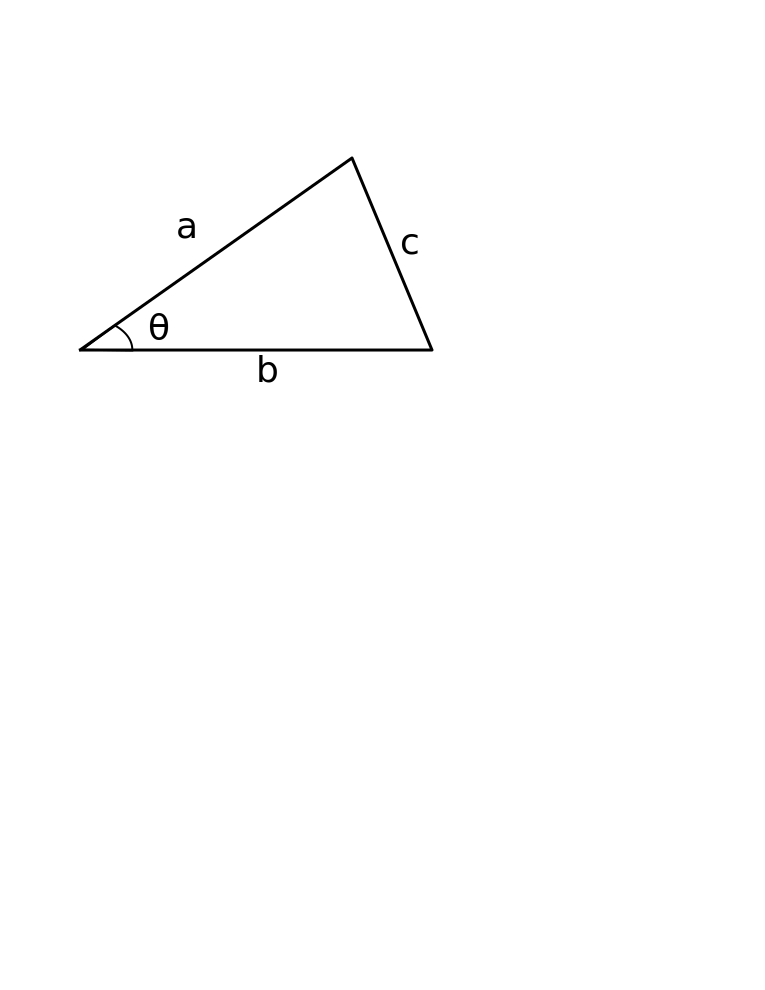
\includegraphics[width=5cm]{ink/week11/lawOfCosines}

  \item Determine the magnitude of the vector
    \begin{eqnarray*}
      \vec{u} & = & u_1 \vec{\imath} + u_2 \vec{\jmath}.
    \end{eqnarray*}

    \vfill

  \item Determine the magnitude of the vector
    \begin{eqnarray*}
      \vec{v} & = & v_1 \vec{\imath} + v_2 \vec{\jmath}.
    \end{eqnarray*}

    \vfill

  \item Determine the magnitude of the vector $\vec{u}-\vec{v}$ using
    the components as described above.
    \sideNote{Determine the components of $\vec{u}-\vec{v}$ and do not
      forget to FOIL out the terms when you determine the magnitude.}

    \vfill

  \end{subproblem}

\end{problem}


\actTitle{The Dot Product}
\begin{problem}
\item  In the diagram below sketch the vector $\vec{u}-\vec{v}$.

  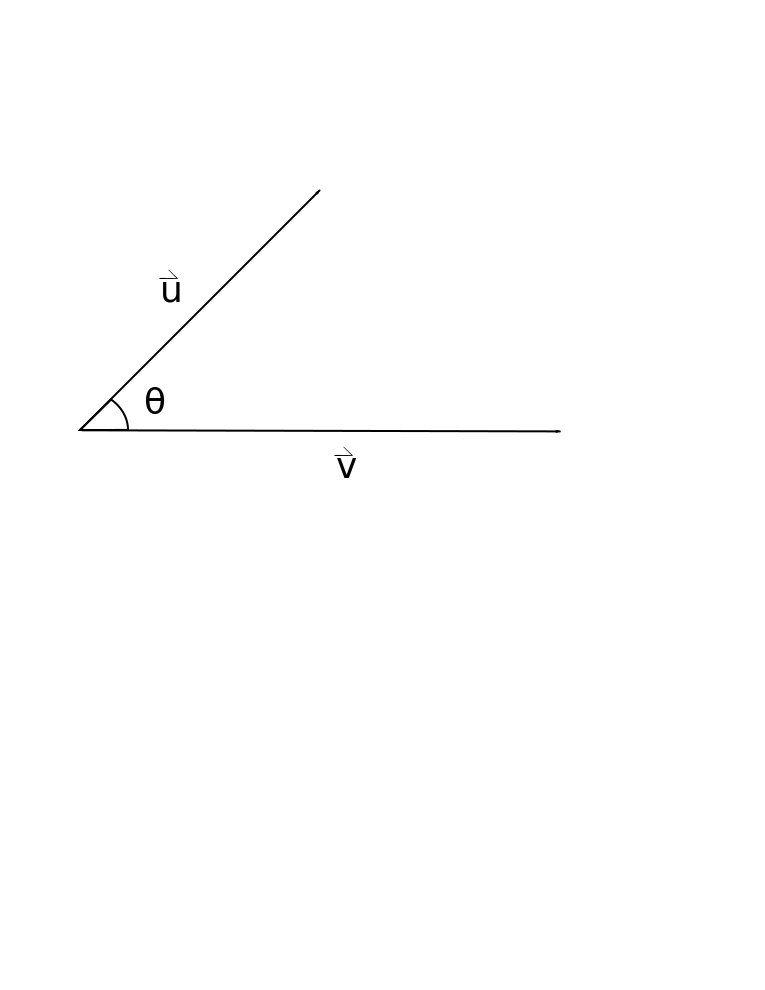
\includegraphics[width=7cm]{ink/week11/dotProduct}

\item Using your results from the pre-class work determine the value
  of
  \begin{eqnarray*}
    \| \vec{u} \| \| \vec{v} \| \cos(\theta)
  \end{eqnarray*}
  in terms of $\|\vec{u}\|$, $\|\vec{v}\|$, and $\|\vec{u}-\vec{v}\|$.

  \vfill

\item Substitute the components for $\vec{u}$ and $\vec{v}$ and
  simplify the expression as much as possible.

  \vfill

\clearpage

\item Determine the component of
  \begin{eqnarray*}
    \vec{u} & = & 5 \vec{\imath} + 3 \vec{\jmath}
  \end{eqnarray*}
  in the direction of
  \begin{eqnarray*}
    \vec{v} & = & \vec{\imath} + 2 \vec{\jmath}.
  \end{eqnarray*}

  \begin{subproblem}
  \item Make a sketch of the two vectors. (Make it big.)
    \vfill
  \item Draw the components on your sketch above.
  \item Calculate the length of the component of $\vec{u}$ in the
    direction of $\vec{v}$.
    \vfill
  \end{subproblem}

\end{problem}


\postClass

\begin{problem}
\item Briefly state two ideas from today's class.
  \begin{itemize}
  \item
  \item
  \end{itemize}
\item
  \begin{subproblem}
    \item
  \end{subproblem}
\end{problem}


%=========================================================================
% Start of activity on the cross product
%=========================================================================
\preClass{The Area of a Parallelogram}

\begin{problem}
\item Determine the area of the parallelogram shown below. The area
  should be in terms of $a$, $b$, and $\theta$.

  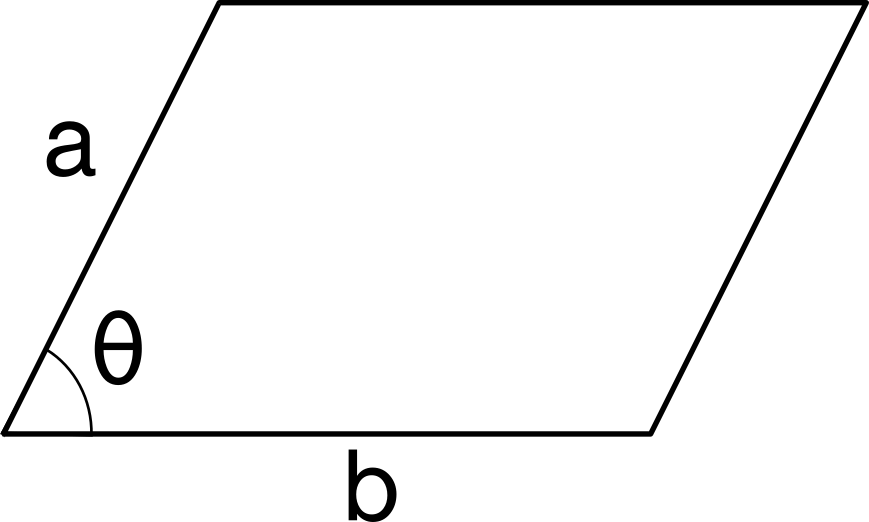
\includegraphics[width=5cm]{ink/week11/parallelogram}

  \vfill

\item Expand the expression
  \begin{eqnarray*}
    \left( a + b \right) \cdot \left( c + d \right).
  \end{eqnarray*}
  \sideNote{FOIL out the product.}

  \vfill

\end{problem}


\actTitle{The Cross Product}
\begin{problem}
\item A new operation, the cross product, is defined, and the
  operations to calculate the cross product are derived. The cross
  product of two vectors, $\vec{u}\times\vec{v}$, is derived by first
  defining the following identities:
  \begin{eqnarray*}
    \vec{\imath} \times \vec{\jmath} & = & \vec{k}, \\
    \vec{\jmath} \times \vec{k} & = & \vec{\imath}, \\
    \vec{k} \times \vec{\imath} & = & \vec{\jmath}, \\
    \vec{u} \times \vec{u} & = & 0 \vec{\imath}, \\
    \vec{u} \times \vec{v} & = & - \vec{v} \times \vec{u}.
  \end{eqnarray*}
  Note that the cross product of two vectors is a vector.
  \begin{subproblem}
  \item For the first three identities above make a sketch to
    demonstrate the relationships.
    \vfill

    \clearpage

  \item Suppose that
    \begin{eqnarray*}
      \vec{u} & = & u_1 \vec{\imath} + u_2 \vec{\jmath}
    \end{eqnarray*}
    and
    \begin{eqnarray*}
      \vec{v} & = & v_1 \vec{\imath} + v_2 \vec{\jmath}.
    \end{eqnarray*}
    Use the definitions above and assume that the cross product obeys
    the distributive rule to derive a general formula for the cross
    product.
    \vfill
    \vfill

  \item Determine the cross product of $2 \vec{\imath} + 2\vec{\jmath}$ and $4 \vec{\imath}$.
    \vfill

    \clearpage

  \item Suppose that
    \begin{eqnarray*}
      \vec{u} & = & u_1 \vec{\imath} + u_2 \vec{\jmath} + u_3 \vec{k}
    \end{eqnarray*}
    and
    \begin{eqnarray*}
      \vec{v} & = & v_1 \vec{\imath} + v_2 \vec{\jmath} + v_3 \vec{k}.
    \end{eqnarray*}
    Use the definitions above and assume that the cross product obeys
    the distributive rule to derive a general formula for the cross product.
    \vfill

  \end{subproblem}
\end{problem}


\postClass

\begin{problem}
\item Briefly state two ideas from today's class.
  \begin{itemize}
  \item
  \item
  \end{itemize}
\item
  \begin{subproblem}
    \item
  \end{subproblem}
\end{problem}


%=========================================================================
% Start of activity on motion in a circle
%=========================================================================
\preClass{Path Around The Unit Circle}

\begin{problem}
\item Suppose that the position of a point mass is given by
  \begin{eqnarray*}
    \vec{r}(t) & = & \cos(t) \vec{\imath} + \sin(t) \vec{\jmath}.
  \end{eqnarray*}
  \begin{subproblem}
  \item Determine the position of the point mass at ${\displaystyle
      t=\frac{\pi}{3}}$.
    \sideNote{Your answer should be a vector using
      $\vec{\imath}-\vec{\jmath}$ notation.}
    \vfill
  \item Determine the position of the point mass at ${\displaystyle
      t=\frac{\pi}{4}}$.
    \vfill
  \item Determine the position of the point mass at ${\displaystyle
      t=\frac{2\pi}{3}}$.
    \vfill
  \item Determine the position of the point mass at ${\displaystyle
      t=\frac{\pi}{2}}$.
    \vfill
    (over)
    \clearpage
  \item Make a sketch of all the points that the point mass moves
    through from $t=0$ to $t=2\pi$. (Mark the starting point and the
    direction of movement.)
    \vfill
  \end{subproblem}
\end{problem}


\actTitle{Angular Velocity}
\begin{problem}
\item Suppose that the position of a point mass is given by
  \begin{eqnarray*}
    \vec{r}(t) & = & R\cos(\theta(t)) \vec{\imath} + R\sin(\theta(t)) \vec{\jmath},
  \end{eqnarray*}
  where $R$ is a constant and $\theta(t)$ is a function of time.
  \label{activity:angularVelocity:one}
  \begin{subproblem}
  \item What can you say about the position of the point mass?
    \vfill
  \item What is the magnitude of the position?
    \vfill
  \item What is the velocity of the point mass in terms of $\theta(t)$
    and $\theta'(t)$.
    \vfill
  \item What is the magnitude of the velocity?
    \vfill
  \end{subproblem}

  \clearpage

\item Assume that a point mass is located on the edge of a circle with
  radius $R$.  From the definition of radian measure the position on
  the arc of a circle is given by
  \begin{eqnarray*}
    s & = & R \theta(t).
  \end{eqnarray*}
  \label{activity:angularVelocity:two}
  \begin{subproblem}
  \item Assume that $R$ is a constant. Determine the speed of the
    point mass.
    \vfill
  \item How do you interpret the meaning of $\theta'(t)$?
    \vfill
  \item Assume that $R$ is a constant. Determine the acceleration of
    the point mass.
    \vfill
  \end{subproblem}

\clearpage

\item Assume that the point masses in questions
  \ref{activity:angularVelocity:one} and
  \ref{activity:angularVelocity:two} above have mass $m$ kg. In both
  cases determine the kinetic energy of the point masses.

\end{problem}


\postClass

\begin{problem}
\item Briefly state two ideas from today's class.
  \begin{itemize}
  \item
  \item
  \end{itemize}
\item
  \begin{subproblem}
    \item
  \end{subproblem}
\end{problem}



%=========================================================================
% Start of activity on riemann sums and moment of intertia
%=========================================================================
\preClass{Moment of Inertia}

\begin{problem}
\item A point mass of 2 kg is located at $3\vec{i} + 2\vec{j}$, and a
  point mass of 4 kg is located at $-\vec{i}+3\vec{j}$. The two masses
  rotate around the $\vec{k}$ axis at the same rate. Determine the
  moment of inertia of inertia of the two masses.

  \vfill

  \clearpage


\item A set of three point masses is lined up on the $x$ axis. They are
  positioned at $x_n=\frac{n}{3}$ where $n=0,~1,~2$. The mass of
  each point mass is $\frac{5n}{3}$ kg.
  \begin{subproblem}
    \item Make a rough sketch of the system.
      \vfill
    \item Determine the center of mass of the system.
      \vfill
    \item Determine the moment of inertia of the system around the
      $y$-axis.
      \vfill
  \end{subproblem}


\end{problem}


\actTitle{Moment of Inertia for Continuous Masses}
\begin{problem}
\item A thin metal rod is located on the $x$-axis. The left side of
  the rod is located at $x=0$m and the right hand side is located at
  $x=1$m. The density of the rod is given by $\rho(x)=5x$ kg/m.
  \begin{subproblem}
    \item Make a rough sketch of the system.
      \vfill
    \item Divide it up into $N$ equal sized small segments. Determine
      the location of the left hand side of each small segment.
      \vfill
    \item Determine an approximation for the density of each small
      segment. (Keep the approximation in terms of $x_k$.)
      \vfill
    \item Determine the approximate mass and the moment of inertia
      around the $y$-axis for each small segment.
      \vfill

      \clearpage

    \item Determine the sum that can be used to approximate the center
      of mass and the sum that can be used to approximate the moment
      of inertia around the $y$-axis.

      \vfill

    \item Determine the center of mass and the moment of inertia for
      the rod.

      \vfill
      \vfill

  \end{subproblem}
\end{problem}

\postClass

\begin{problem}
\item Briefly state two ideas from today's class.
  \begin{itemize}
  \item
  \item
  \end{itemize}
\item Relate the sum for the center of mass with the integral. Make a
  plot and discuss the relationship with the sum with the area under a
  function. (Which function are you finding the area under?)

  \vfill
\end{problem}


%=========================================================================
% Start of day on moment of inertia and angular momentum.
%=========================================================================
\preClass{Constant Angular Velocity}

\begin{problem}
\item An object moves around a circle with a constant angular
  velocity, $\omega$, and a constant distance from the origin,
  $r$. The initial angle, $\theta$, is zero.
  \begin{subproblem}
  \item Determine the angle at any time.
    \vfill
  \item Determine the position at any time.
    \sideNote{Use proper vector notation.}
    \vfill
  \item Determine the derivative of the position at any time.
    \vfill
  \item What is the magnitude of the velocity vector?
    \vfill
  \item Determine the derivative of the velocity at any time.
    \vfill
  \end{subproblem}

  \clearpage

\item An object moves around a circle of radius $r$  at a constant
  rate, $\theta=\omega t$. Its position at any time is $\vec{r}$.

  \begin{subproblem}
    \sideNote{Draw the vector $\delta\vec{r}$ in the plot.}
  \item based on the plot below to graphically represent the
    difference in the positions between any times, $\vec{r}(t+\delta
    t)-\vec{r}(t)$. Blow up, redraw, and focus just on the two
    positions on the circle.

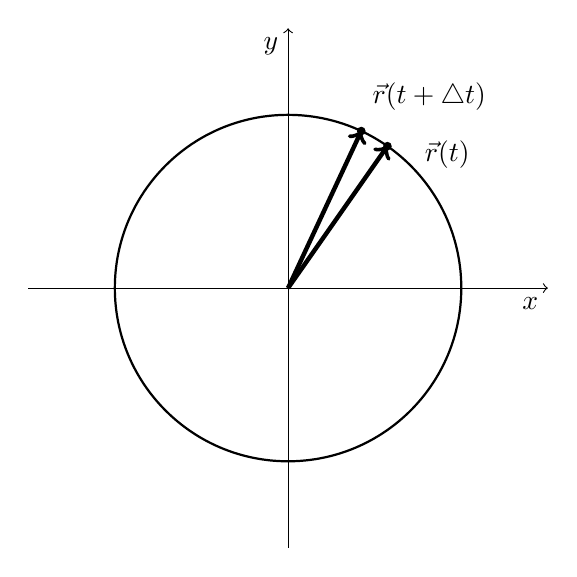
\begin{tikzpicture}[y=2.2cm, x=2.2cm,font=\sffamily]
  \draw[black,->] (-1.5,0) -- (1.5,0) node[anchor=north east] {$x$};
  \draw[black,->] (0,-1.5) -- (0,1.5) node[anchor=north east] {$y$};
  \draw[black,thick] (0,0) circle [radius=1];
  \fill[black,shift={+(55:1)}] (0,0) circle [radius=0.025];
  \fill[black,shift={+(65:1)}] (0,0) circle [radius=0.025];
  \draw[black,->,ultra thick] (0,0) -- +(55:1) node[anchor=west,shift={(0.15,-0.05)}] {$\vec{r}(t)$};
  \draw[black,->,ultra thick] (0,0) -- +(65:1) node[anchor=west,shift={(0,0.2)}] {$\vec{r}(t+\triangle t)$};
\end{tikzpicture}
    \vfill

    \sideNote{Draw the velocity vectors and then sketch the difference.}
  \item Graphically represent the difference in the velocity vectors,
    $\vec{v}(t+\delta t)-\vec{v}(t)$, at the two positions in the plot
    below. Blow up, redraw, and focus just on the two positions on the
    circle.

    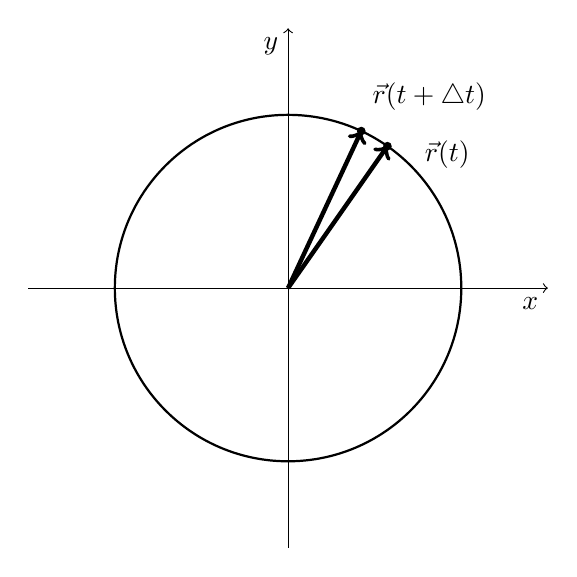
\begin{tikzpicture}[y=2.2cm, x=2.2cm,font=\sffamily]
      \draw[black,->] (-1.5,0) -- (1.5,0) node[anchor=north east] {$x$};
      \draw[black,->] (0,-1.5) -- (0,1.5) node[anchor=north east] {$y$};
      \draw[black,thick] (0,0) circle [radius=1];
      \fill[black,shift={+(55:1)}] (0,0) circle [radius=0.025];
      \fill[black,shift={+(65:1)}] (0,0) circle [radius=0.025];
      \draw[black,->,ultra thick] (0,0) -- +(55:1) node[anchor=west,shift={(0.15,-0.05)}] {$\vec{r}(t)$};
      \draw[black,->,ultra thick] (0,0) -- +(65:1) node[anchor=west,shift={(0,0.2)}] {$\vec{r}(t+\triangle t)$};
    \end{tikzpicture}

    \vfill

  \end{subproblem}

\end{problem}


\actTitle{Energy Associated With Constant Angular Velocity}
\begin{problem}
\item An object moves around a circle of radius $r$  at a constant
  rate, $\theta=\omega t$. Its position at any time is $\vec{r}$.

  \begin{subproblem}
  \item Determine the position at any time. Express the position as
    a vector.
    \sideNote{Assume that $\omega$ is constant.} %\\
    %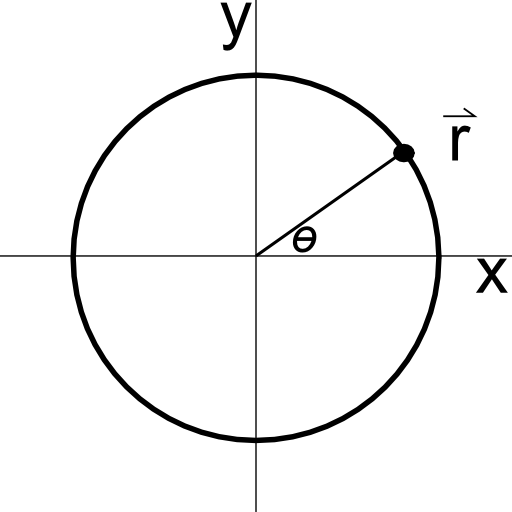
\includegraphics[width=7cm]{ink/week12/circularMotion}
    \vfill
  \item Determine the velocity and the acceleration by taking the
    derivatives of the position with respect to time.
    \vfill
  \item Determine the kinetic energy of the object at any time.
    \vfill
  \end{subproblem}

  \clearpage

\item An object whose position is given by $\vec{r}(t)$ is moving in
  two dimensions. The angle between the velocity and the position is
  $\gamma$ as shown in the diagram below. The velocity can be
  expressed by two components, one in the direction of the position
  vector and the other direction
  perpendicular to the position vector. \\
  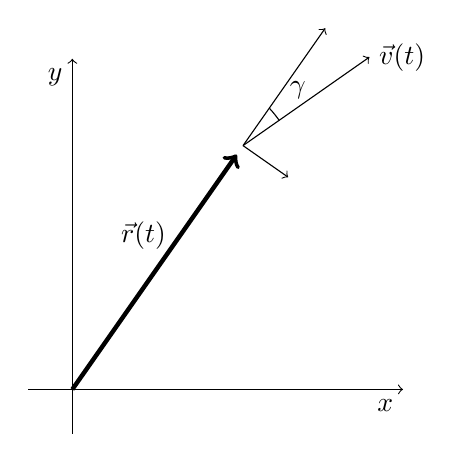
\begin{tikzpicture}[y=2.8cm, x=2.8cm,font=\sffamily]
    \draw[black,->] (-0.2,0) -- (1.5,0) node[anchor=north east] {$x$};
    \draw[black,->] (0,-0.2) -- (0,1.5) node[anchor=north east] {$y$};
    \draw[black,->,ultra thick] (0,0) -- +(55:1.3) node[midway,above,shift={(-0.05,0.05)}] {$\vec{r}(t)$};
    \draw[black,->] (55:1.35) -- +(55:0.65);
    \draw[black,->] (55:1.35) -- +(-35:0.25);
    \draw[black,->] (55:1.35) -- +(35:0.7) node[anchor=west,shift={(0.0,0.0)}] {$\vec{v}(t)$};
    \node at (53:1.7) {$\gamma$};
    \draw (55:1.35) ++(35:0.2) arc(35:43:0.5);
  \end{tikzpicture}

  \begin{subproblem}
  \item Determine the magnitude of the component of the velocity that
    is parallel to the position vector and the magnitude of the
    component of the velocity that is perpendicular to the position
    vector. Your answer should be in terms of the magnitude of
    $\vec{v}$ and the angle between the vectors, $\gamma$.

    \vfill

  \item Determine the magnitude of the vector given by
    $\vec{r}\times\vec{v}$.

    \vfill

  \item Determine the value of $\vec{r}\cdot\vec{v}$ in terms of the
    magnitude of the position and velocity vectors.

    \vfill

  \item Determine the magnitude of the component of the velocity that
    is parallel to the position vector and the magnitude of the
    component of the velocity that is perpendicular to the position
    vector in terms of the dot and cross products above.

    \vfill

  \end{subproblem}
  \clearpage
\item An object moves around a circle of radius $r$  at a constant
  rate, $\theta=\omega t$. Its position at any time is $\vec{r}$.
  \begin{subproblem}
  \item Determine $\vec{r}\times\vec{v}$ and the magnitude of the
    result.

    \vfill

  \item Determine  $\vec{r}\cdot\vec{v}$.

    \vfill

  \item What do these two results imply about the relationship between
    the position and velocity vectors?

    \vfill

  \end{subproblem}
\end{problem}

\postClass

\begin{problem}
\item Briefly state two ideas from today's class.
  \begin{itemize}
  \item
  \item
  \end{itemize}
\item for each image below make a rough sketch of the missing
  component, $\vec{r}$, $\vec{v}$, or $\vec{\omega}$.
  \begin{subproblem}
  \item 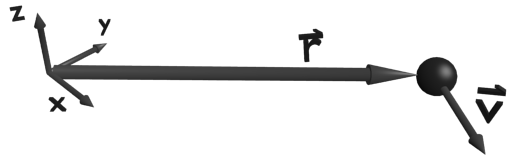
\includegraphics[width=7cm]{blender/week12/negativeZOmega}
  \item 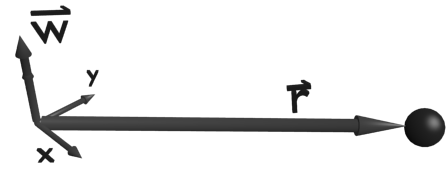
\includegraphics[width=7cm]{blender/week12/findOmega}
  \item 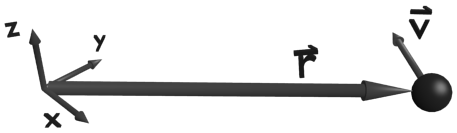
\includegraphics[width=7cm]{blender/week12/positiveZOmega}
  \end{subproblem}
\end{problem}


%=========================================================================
% Start of activity on angular velocity for simple and non-simple
% harmonic motion.
%=========================================================================
\preClass{Constant Angular Velocity}

\begin{problem}
%\item A mass is moving in a circle of radius $R$ at a constant speed,
%  $v$.
%  \begin{subproblem}
%  \item Draw a picture of the path and include the free body diagram.
%    \vfill
%  \item Add the acceleration of the object in your plot above. In
%    which direction is the acceleration?
%    \vfill
%  \item What is the magnitude of the acceleration?
%    \vfill
%  \item How will the diagram change if the velocity is not constant?
%    \vfill
%  \end{subproblem}
%
%\clearpage

\item The position of a mass is
  $\vec{r}(t)=r\cos(\omega t)\vec{i}+r\sin(\omega t)\vec{j}$. The
  value of $\omega$ is a positive constant.
  \begin{subproblem}
  \item Draw a sketch of the object's path. Include the start point
    and the direction of travel of the object.
    \vfill
  \item How long does it take to complete one full revolution?
    \vspace{3em}
  \item Determine the velocity and acceleration. Add a sketch of the
    vectors to your plot above.
    \vfill
    \clearpage
  \item Determine the value of $|\vec{a}(t)|$ using your results for
    the velocity and acceleration above.
    \vfill
  \item Determine the value of $\frac{|\vec{v}(t)|^2}{|\vec{r}(t)|}$
    using your results for the velocity and acceleration above.
    \vfill
  \end{subproblem}

\end{problem}

\actTitle{Non-constant Angular Velocity}
\begin{problem}
\item The position of a mass is
  $\vec{r}(t)=r\cos(\omega t^2)\vec{i}+r\sin(\omega t^2)\vec{j}$. The
  value of $\omega$ is a constant.
  \begin{subproblem}
  \item Draw a sketch of the object's path. Include the start point
    and the direction of travel of the object.
    \vfill
  \item Determine the velocity and acceleration. Add a sketch of the
    vectors to your plot above.
    \vfill
    \clearpage
  \item Is the relationship $|\vec{a}|=\frac{|\vec{v}(t)|^2}{|\vec{r}(t)|}$
    still valid?
    \vfill
    \vfill
  \item Determine the radial component, $\vec{a}_r(t)$, of the
    acceleration.
    \vfill
  \item Show that $|\vec{a}_r(t)| = \frac{|\vec{v}(t)|^2}{|\vec{r}(t)|}$
    \vfill
  \end{subproblem}
\end{problem}

\postClass

\begin{problem}
\item Briefly state two ideas from today's class.
  \begin{itemize}
  \item
  \item
  \end{itemize}
\item The position of a mass is
  $\vec{r}(t)=r\cos(\omega t)\vec{i}+r\sin(\omega t)\vec{j}$. The
  value of $\omega$ is a constant.
  \begin{subproblem}
  \item Draw a sketch of the object's path. Include the start point
    and the direction of travel of the object.
    \vfill
    \vfill
  \item Find the distance that the mass travels from time $t=0$ to a
    later time, $t=T$.
    \vfill
  \item What happens as the value of $\omega$ changes? For example
    if you double $\omega$ what happens to the distance? What does
    that imply about the speed?
    \vfill
  \end{subproblem}
\end{problem}


%=========================================================================
% Start of day on the derivative of inverse functions
%=========================================================================
\preClass{Inverse Trigonometric Functions}

\begin{problem}
\item Make a sketch of the unit circle. Mark and label the points on
  the circle that correspond to the angles $\frac{\pi}{4}$,
  $\frac{\pi}{3}$, and $\frac{3\pi}{4}$.
  \sideNote{Label the angle as well as the points on the edge of the circle.}
  \vfill
  \vfill
\item If the sine of an angle is $\frac{\sqrt{2}}{2}$ what are all
  possible values of the angle?
  \vfill
\item If the sine of an angle is $\frac{\sqrt{3}}{2}$ what are all
  possible values of the angle?
  \vfill
\end{problem}


\actTitle{The Derivative of the Inverse of a Function}
\begin{problem}
\item Suppose that
  \begin{eqnarray}
    \label{eqn:arcsin}
    y &= & \arcsin(t),
  \end{eqnarray}
  and assume that $y$ is between $\frac{-\pi}{2}$ and $\frac{\pi}{2}$ and
  $t$ is between -1 and 1.
  \begin{subproblem}
  \item Solve equation \ref{eqn:arcsin} for $t$ as a function of
    $y$.
    \label{subproblem:inverseSine}
    \vfill
  \item Assuming that $y$ is a function of $t$ use the chain rule to
    determine the derivative of $y(t)$ with respect to $t$.
    \vfill
  \item Use the identity $\sin^2(y)+\cos^2(y)=1$ to express $y'(t)$ in
    terms of $\sin(y)$.
    \vfill
  \item Use the definition of $y(t)$ from part \ref{subproblem:inverseSine} to determine $y'(t)$ only in
    terms of $t$.
    \vfill

  \end{subproblem}

  \clearpage

\item Suppose that
  \begin{eqnarray}
    \label{eqn:inverseFunction}
    y &= & f^{-1}(t).
  \end{eqnarray}
  \begin{subproblem}
  \item Solve equation \ref{eqn:inverseFunction} for $t$ as a function
    of $y$.
    \label{subproblem:generalInverse}
    \vfill

  \item Assuming that $y$ is a function of $t$ use the chain rule to
    determine the derivative of $y(t)$.
    \vfill

  \item Use the definition of $y(t)$ from equation (\ref{eqn:inverseFunction}) to determine $y'(t)$ only in terms of $t$.
    \vfill

  \end{subproblem}


\end{problem}

\postClass

\begin{problem}
\item Briefly state two ideas from today's class.
  \begin{itemize}
  \item
  \item
  \end{itemize}

\item Use the result on the derivative of the inverse to show that the
  derivative of the square root function satisfies
  \begin{eqnarray*}
    \frac{d}{dt} \sqrt{t} & = & \frac{1}{2\sqrt{t}}.
  \end{eqnarray*}

  \vfill

\item Use the result on the derivative of the inverse to determine the
  derivative of the inverse cosine function.
  \vfill

\item Use the result on the derivative of the inverse to show that the
  derivative of the natural logarithm satisfies
  \begin{eqnarray*}
    \frac{d}{dt} \ln(t) & = & \frac{1}{t}.
  \end{eqnarray*}

  \vfill


\end{problem}




%%% Local Variables:
%%% mode: latex
%%% TeX-master: "labManual"
%%% End:
